
\chapter{RESUMEN DE VALORES.} %(((
A continuación, se muestra el detalle del valor razonable de los equipos valuados.
Para aquellos para los cuales se encontró mercado, el valor razonable se obtuvo a partir
de el modelo de regresión lineal múltiple, el cual se llevo a cabo en el Enfoque de Mercado.
Para los otros activos se tomó el V.N.R. obtenido por el enfoque de Costos.

\section{Obtención del Valor Razonable.} % (((
\begin{figure}[hbtp!]
	\centering
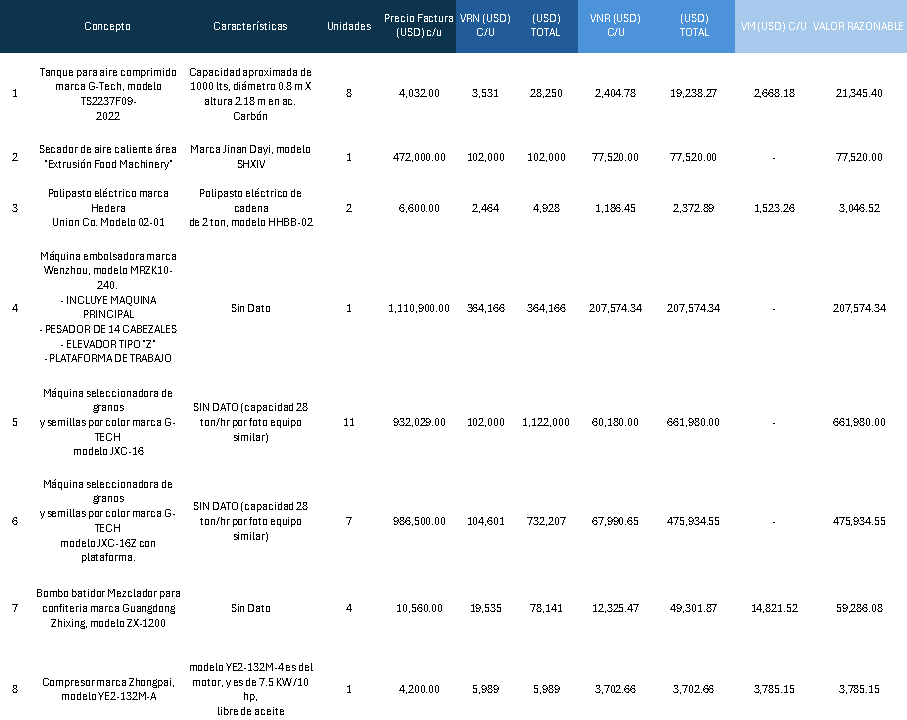
\includegraphics[width=  \linewidth, page = 1]{../0.imagenes/CAP_9/tabla_resumen_1}
\end{figure}
\newpage
\begin{figure}[hbtp!]
	\centering
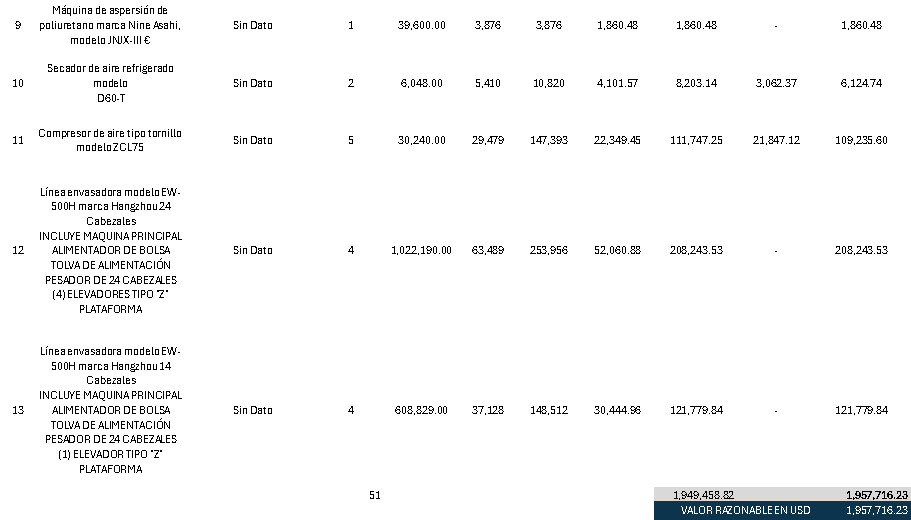
\includegraphics[width=  \linewidth, page = 1]{../0.imagenes/CAP_9/tabla_resumen_2}
\end{figure}
\espacio
% )))

% \begin{table}[hbtp!]
% \begin{tabular}{|*{8}{l|}}
	% \hline 
	% Cetes 28 (Forecast) & \(m\) & 28/18 & meses & años & A/A & VR (USD) & 1,970,951.83 \\ \hline 
	% 0.1025 & 13.04 & 0.007863014 & 12 & 1 & 0.10749324 & TC & 19.28 \\ \hline 
% \end{tabular}
% \end{table}
% 
% \begin{table}[hbtp!]
	% \centering
	% \begin{tabular}{|l|l|}
		% \hline 
		% Comisión Broker & 5\% \\ \hline 
	% \end{tabular}
% \end{table}
% 
% \begin{table}[hbtp!]
	% \centering
	% \begin{tabular}{*{4}{l|}}
		% Renta Bodega/mes & meses & Total & Porcentaje \\ \hline 
		% \$ 100,000.00 MXN & 12 & 1,200,000.00 MXN & 0.03 \\ \hline 
	% \end{tabular}
% \end{table}

% )))
